\documentclass{article}

\usepackage{polski}
\usepackage[margin=1in]{geometry}
\usepackage[parfill]{parskip}
\usepackage{amsmath}
\usepackage{graphicx}
\usepackage{caption}
\usepackage{siunitx}
\usepackage[table,xcdraw]{xcolor}
\usepackage{hyperref}
\usepackage[T1]{fontenc}
\usepackage{comment}
\usepackage{float}
\usepackage{csquotes}

\DeclareSIUnit{\natezenie}{\frac{W}{m^2}}

\begin{document}

\begin{center}
\bgroup
\def\arraystretch{1.5}
\begin{tabular}{|c|c|c|c|c|c|}
	\hline
	EAIiIB & \multicolumn{2}{|c|}{\begin{tabular}{@{}c@{}}Stanisław Borowy \\ Maciej Bobrek \end{tabular}} & Rok II & Grupa 1 & Zespół 5 \\
	\hline
	\multicolumn{3}{|c|}{\begin{tabular}{c}Temat: \\ Ogniwo słoneczne \end{tabular}} & 
	\multicolumn{3}{|c|}{\begin{tabular}{c}Numer ćwiczenia: \\ 134 \end{tabular}} \\
	\hline
	\begin{tabular}{@{}c@{}}Data wykonania \\ 08.01.2023 \end{tabular} & \begin{tabular}{@{}c@{}}Data oddania \\ 09.01.2023 \end{tabular} & 
	\begin{tabular}{c}Zwrot do popr.\\\phantom{data} \end{tabular} & \begin{tabular}{c}Data oddania\\\phantom{data}\end{tabular} &
	\begin{tabular}{c}Data zaliczenia\\\phantom{data}\end{tabular} & \begin{tabular}{c}Ocena\\\phantom{ocena}\end{tabular} \\[4ex]
	\hline
\end{tabular}
\egroup
\end{center}

\section{Wstęp teoretyczny}
\emph{Ogniwem słonecznym} nazywamy urządzenie, które zmienia energię
światła słonecznego na prąd elektryczny. Do jego produkcji używa się
półprzewodnika, najczęściej krzemu, w którym kontakt z fotonem
powoduje przeniesienie elektronów
z pasma walencyjnego do pasma przewodnictwa. Elektrony te są następnie,
przez pole elektryczne warstwy zubożonej, \enquote{wymiatane} w
przeciwnych kierunkach, tworząc prąd elektryczny, który może popłynąć
do obwodu zewnętrznego. 

Jeżeli ogniwo słoneczne połączymy w układ z woltomierzem,
amperomierzem i opornikiem regulowanym to możemy zbadać charakterystykę
prądu przez nie generowanego mierząc pary $(U, I)$ i dla różnych
wartości $R$. Moc prądu wynosi
\begin{align}
    P = UI,
\end{align}
istnieje zatem wartość $R$ dla której iloczyn $U$ i $I$ jest maksymalny
$\Rightarrow$ moc $P$ jest maksymalna. Tę wartość $R$ możemy wyznaczyć ze zbadanej
charakterystyki.

Sprawność ogniwa słonecznego wynosi
\begin{align}
    \eta = \frac{P_{max}}{\phi nS},
    \label{eq:sprawnosc}
\end{align}
gdzie $\phi$ jest natężeniem światła padającego na ogniwo, $n$ liczbą sekcji ogniwa, a $S$
powierzchnią sekcji.
\section{Aparatura}
Do wykonania ćwiczenia zespół użył 
\begin{enumerate}
    \item Fotoogniwo krzemowe: monokrystaliczne, polikrystaliczne i amorficzne. 
    \item Lampę jarzeniową
    \item Amperomierz
    \item Opornicę dekadową
    \item Woltomierz
    \item Luksomierz
\end{enumerate}
Podane wyżej komponenty zostały połączone w następujący układ. Schemat \textbf{a)} przedstawia oświetlenie lampą jarzeniową, a \textbf{b)} układ elektryczny.
\begin{figure}[H]
    \centering
    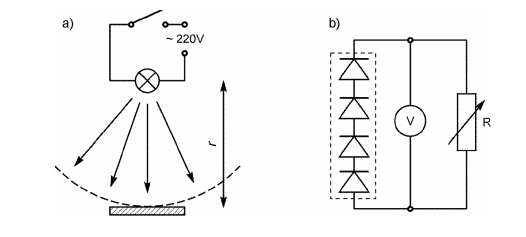
\includegraphics[scale=1]{cw134/schemat_cw134.png}
    \caption{Schemat wykorzystanego układu pomiarowego}
\end{figure}
\section{Wyniki Pomiarów}
Zespół przekręcając pokrętło na oporniku uzyskał kilkanaście punktów pomiarowych
pokrywających zakres napięcia od wartości maksymalnej do bliskiej zeru dla trzech ogniw. Wyniki zebrano w tabeli \ref{pom:1},\ref{pom:2} i \ref{pom:3}.
\begin{table}[!ht]
    \centering
    \begin{tabular}{|l|l|l|l|l|l|l|l|l|l|l|l|l|l|l|l|}
    \hline
        Lp. & 1 & 2 & 3 & 4 & 5 & 6 & 7 & 8 & 9 &10 \\ \hline   %10 & 11 & 12 & 13 & 14 & 15
        I[mA] & 6,4 & 6,3 & 6,2 & 6,1 & 6 & 5,9 & 5,8 & 5,7 & 5,6 & 5,5 \\ \hline   %5,3 & 5,1 & 4,9 & 4,6 & 4,3
        U[V] & 0,011 & 0,277 & 0,545 & 0,83 & 0,982 & 1,15 & 1,278 & 1,407 & 1,439 & 1,47\\ \hline \\ \hline % 1,697 & 1,814 & 1,906 & 2,037 &
         Lp.  & 11 & 12 & 13 & 14 & 15 & & &  & &  \\ \hline
        I[mA]  &5,3 & 5,1 & 4,9 & 4,6 & 4,3 & & & &  &  \\ \hline
        U[V]   & 1,697 & 1,814 & 1,906 & 2,037 & 2,132 & & & &  &   \\ \hline
    \end{tabular}
    \caption{Wyniki pomiarów dla fotoogniwa krzemowego polikrystalicznego}
    \label{pom:1}
\end{table}

Zbadane luksomierzem natężenie światła na wysokości fotoogniwa 
krzemowego polikrystalicznego $\phi = \SI{56.4}{\natezenie}$. 
Dla tego ogniwa ilość sekcji $n = 8$, a powierzchnia sekcji $S= \SI{7.8}{cm^2}$ .

\begin{table}[!ht]
    \centering
    \begin{tabular}{|l|l|l|l|l|l|l|l|l|l|l|}
    \hline
        Lp. & 1 & 2 & 3 & 4 & 5 & 6 & 7 & 8 & 9 & 10 \\ \hline
        I[mA] & 71,3 & 71 & 70,4 & 69,2 & 67,8 & 66 & 62,3 & 55,3 & 48,4 & 38,2 \\ \hline
        U[V] & 0,109 & 0,139 & 0,221 & 0,277 & 0,3 & 0,327 & 0,364 & 0,399 & 0,42 & 0,439 \\ \hline
    \end{tabular}
    \caption{Wyniki pomiarów dla fotoogniwa krzemowego monokrystalicznego}
     \label{pom:2}
\end{table}

Zbadane luksomierzem natężenie światła na wysokości fotoogniwa
krzemowego monokrystalicznego $\phi = \SI{55.5}{\natezenie}$.
Dla tego ogniwa ilość sekcji $n = 1$, a powierzchnia sekcji $S= \SI{63}{cm^2}$ .
\begin{table}[!ht]
    \centering
    \begin{tabular}{|l|l|l|l|l|l|l|l|l|l|l|l|l|}
    \hline
        Lp. & 1 & 2 & 3 & 4 & 5 & 6 & 7 & 8 & 9 & 10 & 11 & 12 \\ \hline
        I[mA] & 1,5 & 1,6 & 1,7 & 1,8 & 1,9 & 2 & 2,1 & 2,2 & 2,3 & 2,4 & 2,5 & 2,6 \\ \hline
        U[V] & 8,904 & 8,835 & 8,687 & 8,523 & 8,336 & 8,072 & 7,92 & 7,369 & 7,058 & 5,476 & 2,311 & 0,01 \\ \hline
    \end{tabular}
    \caption{Wyniki pomiarów dla fotoogniwa krzemowego amorficznego}
 \label{pom:3}
\end{table}

Zbadane luksomierzem natężenie światła na wysokości fotoogniwa
krzemowego amorficznego $\phi = \SI{58.7}{\natezenie}$.
Dla tego ogniwa ilość sekcji $n = 14$, a powierzchnia sekcji $S= \SI{5.5}{cm^2}$ .
\section{Opracowanie wyników pomiarów}
Dla każdego pomiaru została wyliczona uzyskana moc, napięcie na sekcję i gęstość prądu elektrycznego  $\frac{I}{S}$.
Wyniki zebrano w tabelach \ref{obl:1},\ref{obl:2} i \ref{obl:3}.
\begin{table}[H]
    \centering
    \begin{tabular}{|l|l|l|l|l|l|l|l|l|l|l|l|l|l|l|l|}
    \hline
        Lp. & 1 & 2 & 3 & 4 & 5 & 6 & 7 & 8 & 9 &10 \\ \hline   %10 & 11 & 12 & 13 & 14 & 15
        I[mA] & 6,4 & 6,3 & 6,2 & 6,1 & 6 & 5,9 & 5,8 & 5,7 & 5,6 & 5,5 \\ \hline   %5,3 & 5,1 & 4,9 & 4,6 & 4,3
        U[V] & 0,011 & 0,277 & 0,545 & 0,83 & 0,982 & 1,15 & 1,278 & 1,407 & 1,439 & 1,47\\ \hline 
         P[mW] & 0,070 & 1,745 & 3,379 & 5,063 & 5,892 & 6,785 & 7,412 & 8,020 & 8,058 & 8,085 \\ \hline
        U/n[V] & 0,001 & 0,035 & 0,068 & 0,104 & 0,123 & 0,144 & 0,160 & 0,176 & 0,180 & 0,184 \\ \hline
        I/S[mA/cm^2] & 0,821 & 0,808 & 0,795 & 0,782 & 0,769 & 0,756 & 0,744 & 0,731 & 0,718 & 0,705 \\ \hline
        \\ \hline % 1,697 & 1,814 & 1,906 & 2,037 &
         Lp.  & 11 & 12 & 13 & 14 & 15 & & &  & &  \\ \hline
        I[mA]  &5,3 & 5,1 & 4,9 & 4,6 & 4,3 & & & &  &  \\ \hline
        U[V]   & 1,697 & 1,814 & 1,906 & 2,037 & 2,132 & & & &  &   \\ \hline
         
         P[mW] &  8,994 & 9,251 & 9,339 & 9,370 & 9,168 &&&&&\\ \hline
        U/n[V] & 0,212 & 0,227 & 0,238 & 0,255 & 0,267 &&&&&\\ \hline
        I/S[mA/cm^2] & 0,679 & 0,654 & 0,628 & 0,590 & 0,551&&&&& \\ \hline

    \end{tabular}
    \caption{Wyniki obliczeń dla fotoogniwa krzemowego polikrystalicznego}
    \label{obl:1}
\end{table}
\begin{table}[H]
    \centering
    \begin{tabular}{|l|l|l|l|l|l|l|l|l|l|l|}
    \hline
        Lp. & 1 & 2 & 3 & 4 & 5 & 6 & 7 & 8 & 9 & 10 \\ \hline
        I[mA] & 71,3 & 71 & 70,4 & 69,2 & 67,8 & 66 & 62,3 & 55,3 & 48,4 & 38,2 \\ \hline
        U[V] & 0,109 & 0,139 & 0,221 & 0,277 & 0,3 & 0,327 & 0,364 & 0,399 & 0,42 & 0,439 \\ \hline
        P[mW] & 7,77 & 9,87 & 15,56 & 19,17 & 20,34 & 21,58 & 22,68 & 22,06 & 20,33 & 16,77 \\ \hline
        U/n[V] & 0,109 & 0,139 & 0,221 & 0,277 & 0,3 & 0,327 & 0,364 & 0,399 & 0,42 & 0,439 \\ \hline
        I/S[mA/cm\^2] & 1,132 & 1,127 & 1,117 & 1,098 & 1,076 & 1,048 & 0,989 & 0,878 & 0,768 & 0,606   \\ \hline
    \end{tabular}
    \caption{Wyniki obliczeń dla fotoogniwa krzemowego monokrystalicznego}
     \label{obl:2}
\end{table}
\begin{table}[H]
    \centering
    \begin{tabular}{|l|l|l|l|l|l|l|l|l|l|l|l|l|}
    \hline
        Lp. & 1 & 2 & 3 & 4 & 5 & 6 & 7 & 8 & 9 & 10 & 11 & 12 \\ \hline
        I[mA] & 1,5 & 1,6 & 1,7 & 1,8 & 1,9 & 2 & 2,1 & 2,2 & 2,3 & 2,4 & 2,5 & 2,6 \\ \hline
        U[V] & 8,904 & 8,835 & 8,687 & 8,523 & 8,336 & 8,072 & 7,92 & 7,369 & 7,058 & 5,476 & 2,311 & 0,01 \\ \hline
        P[mW] & 13,4 & 14,1 & 14,8 & 15,3 & 15,8 & 16,1 & 16,6 & 16,2 & 16,2 & 13,1 & 5,8 & 0,0 \\ \hline
        U/n[V] & 0,636 & 0,631 & 0,621 & 0,609 & 0,595 & 0,577 & 0,566 & 0,526 & 0,504 & 0,391 & 0,165 & 0,001 \\ \hline
        I/S[mA/cm\^2] & 0,273 & 0,291 & 0,309 & 0,327 & 0,345 & 0,364 & 0,382 & 0,400 & 0,418 & 0,436 & 0,455 & 0,473 \\ \hline
    \end{tabular}
    \caption{Wyniki obliczeń dla fotoogniwa krzemowego amorficznego}
 \label{obl:3}
\end{table}
\newpage
Tworzymy wykres zależności gęstości prądu elektrycznego $\frac{I}{S}$
od napięcia przypadającego na pojedynczą sekcję.

\begin{figure}[H]
    \centering
    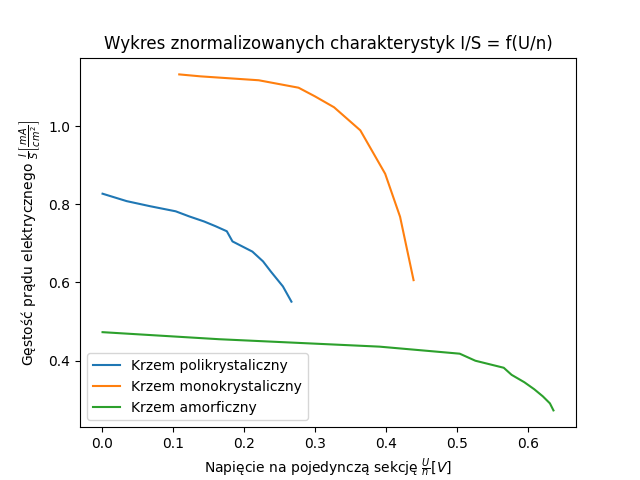
\includegraphics[scale=0.8]{cw134/charakterystyka1.png}
\end{figure}

Najwolniej na nim opada gęstość prądu dla krzemu amorficznego.
Tak więc można ekstrapolować, że posiada on największą gęstość prądu
zwarcia, które daje największe napięcie przypadające na jedną sekcję.

Jako maksymalną moc uzyskaną z fotoogniw przyjmiemy największą
wartość z uzyskanych pomiarów. Tak więc moc maksymalna krzemu
polikrystalicznego wynosić będzie $P_{Amax} = \SI{9.370}{mW}$,
krzemu monokrystalicznego $P_{Bmax} = \SI{22.68}{mW}$, a krzemu
amorficznego $P_{Cmax} = \SI{16.6}{mW}$.  Podstawiając te wartości do
\eqref{eq:sprawnosc} wraz ze zmierzonymi natężeniami światła obliczamy sprawność fotoogniw.
\begin{align*}
    \eta_A &= \frac{9.370 \cdot 10^{-3}}{56.4 \cdot 62.4 \cdot 10^{-4}}
    \cdot 100\% = 2.66\% \\
    \eta_B &= \frac{22.68 \cdot 10^{-3}}{55.5 \cdot 63 \cdot 10^{-4}}
    \cdot 100\% = 6.49\% \\
    \eta_C &= \frac{16.6 \cdot 10^{-3}}{58.7 \cdot 77 \cdot 10^{-4}}
    \cdot 100\% = 3.68\% \\
\end{align*}

\section{Wnioski}
Podłączając 3 różne fotoogniwa do prostego obwodu z regulowanym
opornikiem, amperomierzem i woltomierzem udało nam się wyznaczyć
ich charakterystykę prądowo-napięciową a z niej, ich maksymalną moc
oraz odpowiadającą im sprawności
\begin{enumerate}
    \item Krzem polikrystaliczny -- $P_{max} = \SI{9.370}{mW}$ i
    $\eta = 2.66\%$
    \item Krzem monokrystaliczny -- $P_{max} = \SI{22.68}{mW}$ i
    $\eta = 6.49\%$
    \item Krzem amorficzny -- $P_{max} = \SI{16.6}{mW}$ i
    $\eta = 3.68\%$.
\end{enumerate}

\end{document}
